%-------------------------
%device-revisited.tex
%(c) H.Buchmann FHNW 2018
%export TEXINPUTS=${HOME}/fhnw/edu/:${HOME}/fhnw/edu/tinL/config/latex:${HOME}/fhnw/edu/config//:
%-------------------------
\documentclass{beamer}
\usepackage{latex/beamer}
%---------------------
%local defines
%(c) H.Buchmann FHNW 2009
%$Id$
%---------------------
\newcommand{\target} {\beaglebone\xspace}
\newcommand{\targetS}{{\bf BBG}\xspace}
\newcommand{\host}   {{\em Host}\xspace}
\newcommand{\targetroot} {{\bf target-root}\xspace}
\newcommand{\kernel} {{\bf kernel}\xspace}
\renewcommand{\c}{{\bf C}\xspace}
\newcommand{\cpp}{{\bf C++}\xspace}
\newcommand{\posix}{{\bf POSIX}\xspace}

\input{/home/buchmann/latex/dirtree/dirtree.tex}
\usepackage{svg}
\usepackage[absolute]{textpos}
\setlength{\TPHorizModule}{1mm}
\setlength{\TPVertModule}{1mm}

\begin{document}


\newcommand{\ksp}{{\em kernel-space}}
\newcommand{\usp}{{\em user-space}}

\title[Devices revisited]{Devices revisited}

\frame{\titlepage}

\begin{frame}{Um was geht es ?}{\c und Scripts}
 \begin{itemize}
  \item Verbindung 
  \begin{itemize}
   \item \ksp $\leftrightarrow$ \usp
  \end{itemize}
  \item call-backs
  \begin{itemize}
   \item verschiedene Formen
  \end{itemize}
  \item Info \url[http]{lxr.free-electrons.com}
  \item Schritt f�r Schritt mit \cod{git}
  \begin{itemize}
   \item \cod{git log}
   \item \cod{git show}
  \end{itemize}
 \end{itemize}
\end{frame}

\begin{frame}{Um was geht es ?}
 \begin{itemize}
  \item Kernel-Modules: {\bf L}oadable {\bf K}ernel {\bf M}odule
  \begin{itemize}
   \item \cod{insmod}
   \item \cod{rmmodule}
  \end{itemize}
  \item device
  \begin{itemize}
   \item {\em major} {\em minor}
   \item \cod{devicefile} $=$ {\em major} {\em minor}
  \end{itemize}
  \item \ksp $\leftrightarrow$ {\bf devicefile} $\leftrightarrow$ \usp
 \end{itemize}
\end{frame}

\begin{frame}{Um was geht es ?}{kernel-space $\leftrightarrow$ user-space}
\begin{block}{Wie merkt der {\em kernel}-space}
\begin{itemize}
 \item ob ein {\bf LKM}
 \begin{itemize}
  \item eingef�gt
  \item entfernt 
 \end{itemize}
 wird
\end{itemize}
\end{block}
\begin{block}{Wie merkt der {\em user}-space}
 \begin{itemize}
  \item ob sich in einem {\bf LKM}
  \begin{itemize}
   \item etwas tut  
  \end{itemize}
  wird
 \end{itemize}
\end{block}
\end{frame}

\begin{frame}{Setup}{Programmentwicklung}
\begin{tabular}{l|l}
\multicolumn{1}{c|}{\host} & \multicolumn{1}{c}{\targetS}\\
\hline
start				& \\
\cod{minicom -D/dev/ttyUSB0} 	&\\
				& start\\
        			& \cod{ifconfig usb0 192.168.7.7}\\
        			& \cod{/sbin/sshd}\\
\cod{ssh root@192.168.7.7}      &\\
\cod{sshfs root@192.168.7.7: mount} &\\
\hline
\multicolumn{2}{c}{ready to develop}	
\end{tabular}
\end{frame}

\section{simple-device-*.c:Schritt f�r Schritt}
\begin{frame}{\cod{simple-device-*.c}}{Schritt f�r Schritt}
 \begin{itemize}
  \item \cod{simple-device-1.c}:
  \begin{itemize}
   \item debug mit \cod{printk}
   \item call-back: init/exit
   \item \cod{struct file\_operations}
  \end{itemize}
  \item \cod{simple-device-2.c}:
  \begin{itemize}
   \item call-back: \cod{read/write} fast ohne code
   \item device File: Verbindung 
  \end{itemize}
  \item \cod{simple-device-3.c}:
  \begin{itemize}
   \item das Zusammenspiel der Parameter: \cod{len} und \cod{ofs}
  \end{itemize}
  \item \cod{simple-device-3.c}
  \begin{itemize}
   \item Verbindung mit \usp, das Verzeichnis \cod{/sys}
  \end{itemize}
 \end{itemize}
\end{frame}

\subsection{simple-device-1.c}
\begin{frame}{\cod{simple-device-1.c}}
  \begin{itemize}
   \item init/exit
   \item \cod{struct file\_operations fops;}
   \item include file: \cod{linux/fs.h} im kernel code
  \end{itemize}
  
\end{frame}

\begin{frame}[fragile]{Code}{\cod{linux/fs.h}}
\begin{lstlisting}
struct file_operations {
/* ... */
 ssize_t (*read) (struct file *, 
                  char __user *, 
                  size_t, 
                  loff_t *);
 ssize_t (*write) (struct file *, 
                   const char __user *, 
                   size_t, 
                   loff_t *);
 /*... */
} __randomize_layout;
\end{lstlisting}
\remark{Was ist \cod{\_\_randomize\_layout} ?}
\end{frame}

\begin{frame}[fragile]{Code}
\begin{lstlisting}
/* the call backs defined and **initialized** */
static struct file_operations fops =  
{
 /* do nothing for the moment*/
};

/* init */
 Major = register_chrdev(0, DEVICE, &fops);
/* exit */
 unregister_chrdev(Major,DEVICE);

  \end{lstlisting}
\end{frame}


\subsection{simple-device-2.c}
\begin{frame}{\cod{simple-device-2.c}}{empty read/write}
 \begin{itemize}
  \item {\em kernel-space}
  \begin{itemize}
  \item \cod{file\_operations}: read/write
  \begin{itemize}
   \item mit \cod{printk} call-back anzeigen
  \end{itemize}
  \item verschiedene \cod{return} Werte für read/write
  \end{itemize}
  \item {\em user-space}
  \begin{itemize}
  \item \cod{mknod device c {\em Major} 0} 
  \item read: \cod{cat device}
  \item write wenig Bytes \cod{echo abcd > device} 
  \item viel Bytes \cod{cat file > device}
  \end{itemize}
 \end{itemize}
\end{frame}

\begin{frame}[fragile]{Code}
 \begin{lstlisting}
 printk("simple_read len=%d= *ofs= %lld buffer*=0x%p\n",
                         len,      *ofs,          buffer);
 \end{lstlisting}
\remark{wie \cod{printf} im \usp}
\begin{lstlisting}
static struct file_operations fops =  /* the call backs */
{
 read :simple_read, /* register call-backs */
 write:simple_write,
};
\end{lstlisting}
\end{frame}


\subsection{simple-device-3.c}
\begin{frame}{\cod{simple-device-3.c}}{read/write}
\begin{itemize}
 \item read/write:
 \begin{itemize}
  \item \cod{copy\_to\_user}/\cod{copy\_from\_user}
  \item das Zusammenspiel:
  \begin{itemize}
   \item \cod{len} und \cod{*ofs}
  \end{itemize}
 \end{itemize}
\end{itemize}
\end{frame}

\begin{frame}[fragile]{read}
\begin{center}
 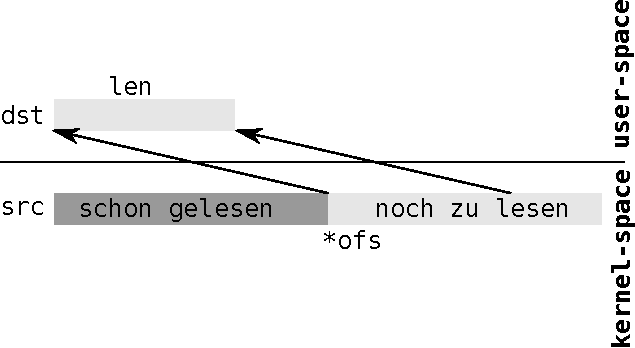
\includegraphics[width=0.875\textwidth]{user-kernel-space-read.pdf}
\end{center}
\vspace{-1.5cm}
\begin{lstlisting}
unsigned long copy_to_user(void __user *to, 
                           const void *from, 
                           unsigned long n)
\end{lstlisting}
\end{frame}

\begin{frame}[fragile]{write}
\begin{center}
 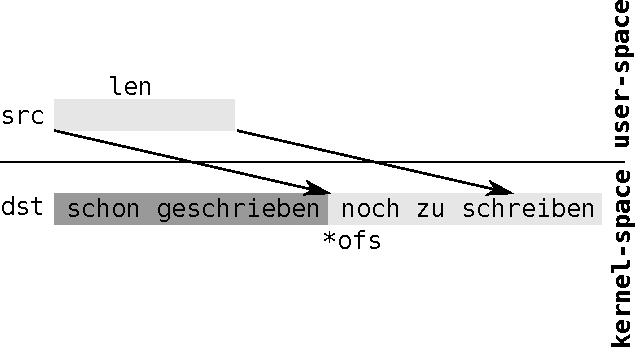
\includegraphics[width=0.875\textwidth]{user-kernel-space-write.pdf}
\end{center}
\vspace{-1.5cm}
\begin{lstlisting}
unsigned long copy_from_user(void *to, 
                                 const void __user *from, 
                                 unsigned long n)
\end{lstlisting}
\end{frame}


\subsection{simple-device-4.c}
\begin{frame}{\cod{simple-device-4.c}}{Verbindung mit {\em userspace}: \cod{/sys}}
\begin{itemize}
 \item {\em kernel-space}
 \begin{itemize}
  \item \cod{MODULE\_LICENSE ("{}GPL"{})}
  \item init: \cod{simple\_module=class\_create(THIS\_MODULE,"{}simple\_device"{})}
  \item exit: \cod{class\_destroy(simple\_class)}
 \end{itemize}
 \item {\em user-space}
 \begin{itemize}
  \item \cod{ls /sys/class}
 \end{itemize}
 \item noch keine Informationen in \cod{/sys/class/simple\_device}
\end{itemize}
\end{frame}



\subsection{simple-device-5.c}
\begin{frame}{\cod{simple-device-5.c}}{Verbindung mit {\em userspace}: \cod{/sys}}
 \begin{itemize}
  \item {\em kernel-space}
  \begin{itemize}
   \item init: \cod{device\_create}, \cod{MKDEV(Major,0)}
   \item exit: \cod{device\_destroy}
  \end{itemize}
  \item {\em user-space}
  \begin{itemize}
   \item \cod{ls /sys/class/simple\_device}
  \end{itemize}
 \end{itemize}
\end{frame}

\begin{frame}[fragile]{Code}
\begin{lstlisting}
struct device *device_create(struct class *cls, 
                             struct device *parent,
			     dev_t devt, 
                             void *drvdata,
			     const char *fmt, ...);

void device_destroy(struct class *cls, 
                    dev_t devt);
\end{lstlisting}
\end{frame}

\begin{frame}{Die Files}{\cod{/sys/class/simple\_device/simple\_device0/}}
\begin{itemize}
 \item der File
 \begin{itemize}
  \item \cod{uevent}
 \end{itemize}
\end{itemize}
\end{frame}

\begin{frame}[fragile]{Die Reihenfolge}
\begin{block}{Beim \cod{init}}
\begin{lstlisting}
 simple_class=class_create(...);
 Major       = register_chrdev(...);
 dev         =device_create(...);
\end{lstlisting}
\end{block}
\begin{block}{Beim \cod{exit}}
 \begin{itemize}
  \item Umgekehrt
 \end{itemize}
\end{block}
\end{frame} 



\begin{frame}{hotplug}
\end{frame}
\end{document}
